\section{GPQA: A Graduate-Level Google-Proof Question and Answer Benchmark}
{{\footnotesize
\begin{description}[labelwidth=5em, labelsep=1em, leftmargin=*, align=left, itemsep=0.3em, parsep=0em]
  \item[date:] 2023-11-20
  \item[version:] TODO
  \item[last\_updated:] 2023-11
  \item[expired:] unknown
  \item[valid:] yes
  \item[valid\_date:] TODO
  \item[url:] \href{https://arxiv.org/abs/2311.12022}{https://arxiv.org/abs/2311.12022}
  \item[doi:] TODO
  \item[domain:] Science (Biology, Physics, Chemistry)
  \item[focus:] Graduate-level, expert-validated multiple-choice questions hard even with web access
  \item[keywords:]
    - Google-proof
    - multiple-choice
    - expert reasoning
    - science QA
  \item[summary:] Contains 448 challenging questions written by domain experts, with expert accuracy at 65\% (74\% discounting clear errors) and non-experts reaching just 34\%. GPT-4 baseline scores \textasciitilde{}39\%-designed for scalable oversight evaluation. :contentReference[oaicite:2]\{index=2\}

  \item[licensing:] TODO
  \item[task\_types:]
    - Multiple choice
  \item[ai\_capability\_measured:]
    - Scientific reasoning
    - knowledge probing
  \item[metrics:]
    - Accuracy
  \item[models:]
    - GPT-4 baseline
  \item[ml\_motif:]
    - Multiple choice
  \item[type:] Benchmark
  \item[ml\_task:]
    - Multiple choice
  \item[solutions:] TODO
  \item[notes:] Google-proof, supports oversight research.

  \item[contact.name:] David Rein (NYU)
  \item[contact.email:] unknown
  \item[datasets.links.name:] GPQA dataset
  \item[datasets.links.url:] \href{zip/HuggingFace}{zip/HuggingFace}
  \item[results.links.name:] ChatGPT LLM
  \item[fair.reproducible:] Yes
  \item[fair.benchmark\_ready:] Yes
  \item[ratings.software.rating:] 0
  \item[ratings.software.reason:] Not analyzed.

  \item[ratings.specification.rating:] 9.0
  \item[ratings.specification.reason:] Clear dual-modality task (image + time-series); environmental focus is well described.

  \item[ratings.dataset.rating:] 9.0
  \item[ratings.dataset.reason:] Time-series and satellite imagery data provided; sensor info and collection intervals are explained.

  \item[ratings.metrics.rating:] 9.0
  \item[ratings.metrics.reason:] ROC-AUC, Precision/Recall are appropriate and robust.

  \item[ratings.reference\_solution.rating:] 1.0
  \item[ratings.reference\_solution.reason:] No starter model or baseline code linked

  \item[ratings.documentation.rating:] 6.5
  \item[ratings.documentation.reason:] Moderate Codabench documentation with climate context; lacks pipeline-level walkthrough.

  \item[id:] gpqa\_a\_graduate-level\_google-proof\_question\_and\_answer\_benchmark
  \item[Citations:] \cite{rein2023gpqagraduatelevelgoogleproofqa}
  \item[Ratings:]
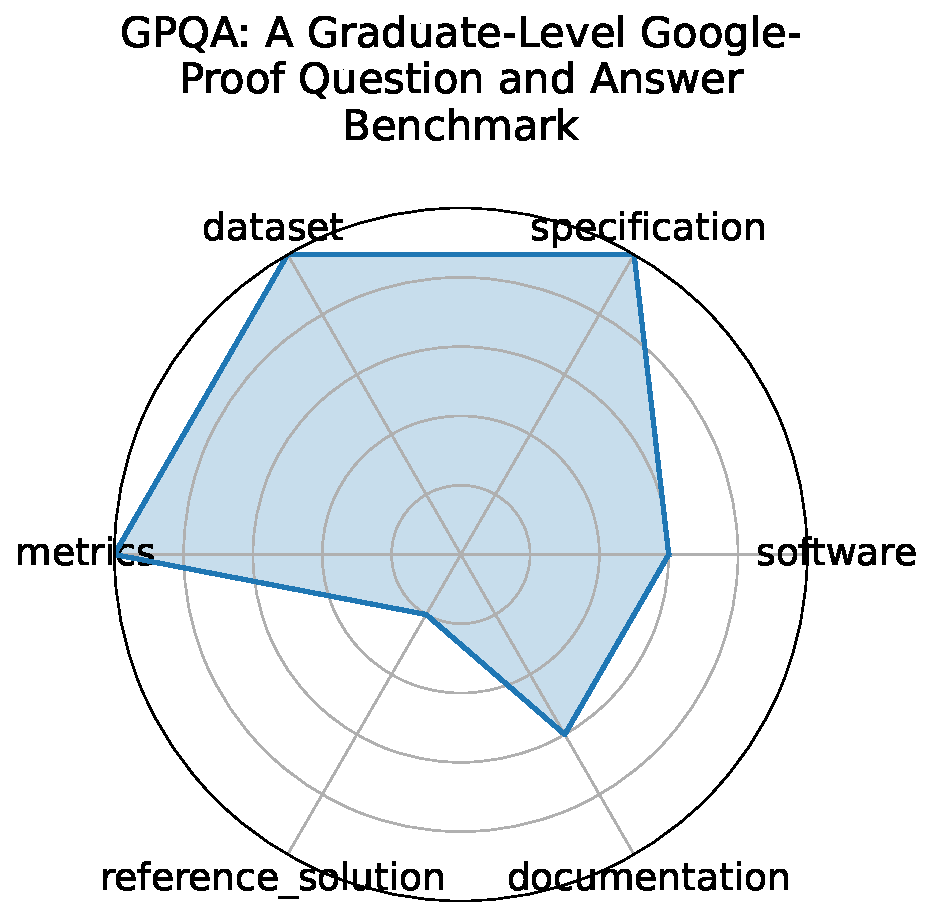
\includegraphics[width=0.2\textwidth]{gpqa_a_graduate-level_google-proof_question_and_answer_benchmark_radar.pdf}
\end{description}
}}
\clearpage